\documentclass[conference]{IEEEtran}

\usepackage{geometry}
\usepackage{graphicx}
\geometry{letterpaper,
top=0.75in,
bottom=1in,
left=0.625in,
right=0.635in
}

 

%% IEEE CNS addition: 
\makeatletter
\def\ps@headings{%
\def\@oddhead{\mbox{}\scriptsize\rightmark \hfil \thepage}%
\def\@evenhead{\scriptsize\thepage \hfil \leftmark\mbox{}}%
\def\@oddfoot{}%
\def\@evenfoot{}}
\makeatother
\pagestyle{empty}

\title{Replication Strategies to Increase Storage Robustness in Decentralized P2P Architectures}
%
%
% author names and IEEE memberships
% note positions of commas and nonbreaking spaces ( ~ ) LaTeX will not break
% a structure at a ~ so this keeps an author's name from being broken across
% two lines.
% use \thanks{} to gain access to the first footnote area
% a separate \thanks must be used for each paragraph as LaTeX2e's \thanks
% was not built to handle multiple paragraphs
%

\author{Brendan Benshoof}

\begin{document}
\maketitle

% note the % following the last \IEEEmembership and also \thanks -
% these prevent an unwanted space from occurring between the last author name
% and the end of the author line. i.e., if you had this:
%
% \author{....lastname \thanks{...} \thanks{...} }
%                     ^------------^------------^----Do not want these spaces!
%
% a space would be appended to the last name and could cause every name on that
% line to be shifted left slightly. This is one of those "LaTeX things". For
% instance, "\textbf{A} \textbf{B}" will typeset as "A B" not "AB". To get
% "AB" then you have to do: "\textbf{A}\textbf{B}"
% \thanks is no different in this regard, so shield the last } of each \thanks
% that ends a line with a % and do not let a space in before the next \thanks.
% Spaces after \IEEEmembership other than the last one are OK (and needed) as
% you are supposed to have spaces between the names. For what it is worth,
% this is a minor point as most people would not even notice if the said evil
% space somehow managed to creep in.



% The paper headers
% The only time the second header will appear is for the odd numbered pages
% after the title page when using the twoside option.
%
% *** Note that you probably will NOT want to include the author's ***
% *** name in the headers of peer review papers.                   ***
% You can use \ifCLASSOPTIONpeerreview for conditional compilation here if
% you desire.




% If you want to put a publisher's ID mark on the page you can do it like
% this:
%\IEEEpubid{0000--0000/00\$00.00~\copyright~2015 IEEE}
% Remember, if you use this you must call \IEEEpubidadjcol in the second
% column for its text to clear the IEEEpubid mark.



% use for special paper notices
%\IEEEspecialpapernotice{(Invited Paper)}




% make the title area


% As a general rule, do not put math, special symbols or citations
% in the abstract or keywords.
\begin{abstract}
Classic P2P key-value storage systems use a small section of strategies to ensure that records are maintained in the system despite constant churn.
These strategies see effective levels of robustness to churn, however they often do not provide effective robustness against systemic failures due to natural disasters and network partitioning in the Internet or the overlay topology of the P2P systems.
We explore and evaluate the status quo of replica robustness strategies in the face of partition failures and propose new techniques to improve over the established methods.
\end{abstract}



\section{Introduction}

In this paper, we will consider a selection of strategies to increase robustness of storage in a p2p network.
Each strategy will be described, analyzed and finally compared and contrasted with other strategies.


Current DHTs are oprimized to store a large number of smaller records.
While is it is perfectly viable to link together such records to store larger files (and even use it as a shared file system), it has generally been used as a layer of indirection and provides means of discovering high bandwidth protocols. For example, Bitorent uses a DHT to help find peers for particular torrent rather than storing the files directly on the DHT.
If we maintain this trend of only storing small records on the DHT, it stands out as a clear choice for use a shared DNS cache, or as a mechanism for storing encrypted cryptographic keys.
All of these  use cases are predicated on a DHT being a reliable store of data.

\section{Technical Background}
\subsection{What is a DHT?}
At the core of maintaining a distributed system is establishing a shared state in the form of a table of key-value pairs.
DHTs provide a mechanism for agreeing upon a very large shared state with tolerable inconsistency (records are sometimes lost, and if mutable they may be inconsistent in value).
While other techniques of concensus provide higher confidance, DHTs scale to awesome levels of storage capacity because they are highly tolerant of the failure of nodes within themselves.
In practice, DHTs and similar distributed system's performance are bound by the CAP Theorem\cite{brewer2010certain}.

As partition tolerance is required in a DHT for long term operation, this leaves us a trade-off between Consistency and Availability.
In DHTs consistency is limited to assure availability of records to users, however such trade-offs are not binary, and we can can seek a balance between availability and consistency to best suit the needs of applications.


\subsection{What are the currently existing DHTs?}

Chord and Kademlia are the most commonly used DHTs in practice. 
Chord has been favored by researchers because it was designed with a series of proofs to show it's consistency in the face of churn.
Sadly these proofs have been shown to be incorrect\cite{} without serious modification to the established protocol.

\subsubsection{Kademlia}

Kademlia is the most popular DHT methodology. 
It powers the trackerless bittorent mainline DHT, and the C implementation related to that project is likely the greatest cause of it's popularity.
many other distributed systems utilize modified versions of Kademlia as a means of peer management and as a key-value store.

Kademlia is built in a non-eucldian metric space. 
Locations are represented by a large integer (160 bit is most common) and the distance between locations is calculated by the XOR metric.
This means Kademlia's metric space is a generalization of a binary tree, where the locations are mapped to leaf nodes and distance between nodes is the distance required to traverse between them on that tree.

Because of the geometric awkwardness of it's metric, Kademlia uses a modified k-nearest neighbors approach to approximate node's voronoi regions and Delaney peers.
If nodes are evenly distributed through the space, kademlia's metric provides an $O(log(n))$ diameter network.

\subsubsection{Chord}

Chord is a familiy of ring-based DHT's.
Locations are represented by a large integer similar to kademlia.
The metric is a unidirectional (bidirectional in some variants) modulus ring.

Chord tracks the immediate peers in either direction on this ring to maintain the networks and calculating delaunay triangulation and voronoi regions in this metric is trivial.

This metric alone would give chord's topology an $O(n)$ diameter 
and to mitigate this, each node maintains $O(log(n))$ ``fingers''
 distributed in such a way that the diameter of the network is reduced to $O(log(n))$.

\subsection{What are DHTs used for}

DHTs are designed to be used to store data in a distributed system that would normally be centrally stored in other systems, like a database or other records.
In practice, they also double as a mechanism for peers discovery and network management.
Many p2p services use a DHT as part of their infrastructure: Bitorrent\cite{jimenez2011kademlia}, CJDNS\cite{hodson2013meshnet}, and I2P\cite{zantout2011i2p}
% %Give examples of how DHTs are used in those projects

\section{Robustness}

\subsection{Robustness and Churn}
Most DHTs focus their efforts on preventing record loss due to churn.
Records are lost to churn under two conditions: the node hosting the replica leaves the network or the node with a replica ceases to be responsible for the record due to a new node joining the network and claiming that portion of the address space. 
We will describe churn as a ``Replacement ratio'': $R_{c}$, which is measured over a period of time (most often a day).
This value describes the portion of DHT's metric space that is maintained by a different node at the end of the period.
This value is related to the more conventional churn rate metric $\frac{exits + joins}{2*size}$ but provides more information on the viability of records.

\subsection{Robustness and network partitions}
Network partitions are when a failure results in the network separating into multiple non-connected networks.
This can be a result of failures in the underlay and the overlay networks.
The result of this, is that unlike the churn based failures, failure of nodes is not independent.
For example, if two previously connected regions of the Internet cease to be connected due to disaster or political intervention, there will be two new networks, each having just lost all nodes in the other partition simultaneously.
This means that robustness methods based periodically re-storing records after they are lost are likely to be insufficient as all the possessors of a record may be found only in one of the partitions.

In practice, overlay partitions may occur due to eclipse attacks and logic errors in how the DHT constructs the overlay.
We will discuss overlay partitions in terms of a ratio $R_{o}$ that describes the size of a connected subnetwork that remains after a partition.
It is worth considering, that in the case of any partition, the ideal behavior is that both resulting partitions remain connected, search-able, and retain findable replicas of all records.


\subsubsection{Underlay Partitions}
An underlay partition can happen as result in a failure of infrastructure, manipulation of BGP, or governmental action.
Assuming the overlay network of the DHT has been constructed randomly in relation to the underlay network, the failures due to the underlay partition will essentially occur at random locations in the network. 

While this may resemble how failure occurs during churn, the failures will all occur effectively simultaneously, to a potentially very large segment of the population of the network.
Kademlia's topology is likely to recover from such an event, however searching the network will be impaired while new connections are established.
Chord's consistent topology proof is built upon an invariant that any join or exit from the network is occurring when the majority of the network is consistent. 
The sudden failure of nodes in a Underlay partition situation violates this assumption and may destroy the ability of the remaining chord networks to form a searchable overlay topology.

We will discuss underlay partitions in terms of a ratio $R_{u}$ that describes the fraction of randomly distributed members of the network that remain after an underlay partition occurs. 

\section{Passive Replication Strategies}

Passive strategies are those where a client writes the record and replicas to the DHT once, then no participant ever re-publishes the record.
Because of constant churn, such records are likely doomed to be lost as the nodes to which they were stored leave the network due to churn.
Because partition failures are being analyzed as specific events, rather than behavior over time, passive strategies will often fair similarly to active strategies because there will not have been sufficient time for nodes or sponsors to take action in response to the partition (If they realize a partition has occurred at all).

\subsection{K-Random Replicas}
The K-random node strategy is not used by any established DHT, however it provides a simple analytical model, which we can extend to the other replica strategies.
In the K-random node strategy, a file is stored at K locations chosen by chaining of a cryptographic hash.
That is, if a record is stored a location $L$, the first replica will be stored at location $hash(L)$ and the second at $hash(hash(L))$ and similarly re-hashing the identifier from the previous step until K nodes have been stored.

This scheme allows for simple speedup and redundancy.
Given a location $L$, any node can locate the potential k backup sites and search them by order of closeness or in parallel (effectively in order of latency).
Because the locations are effectively random, we can simplify our analysis for churn and partition tolerance.

The half-life due to churn for the record (a time period over which, on average, the number of replicas in the network will be halved ) is $\frac{-\log(2)}{\log{1-R_{c}}}$ and because records are a small integer, we can also consider an expected mean lifetime of a record in the network: $\frac{\log{K}}{\log(2)} * \frac{-\log(2)}{\log{1-R_{c}}}$. This value describes the time period after which the expected mean number of remaining replicas is 1. Because this 1 is the mean value, there is a 50\% likelihood there are less than 1 replica (or zero replicas, as the number of replicas is a natural number that cannot take partial values.)

This means we can present the average lifetime of a record in the network in terms of the number of replicas and churn replacement rate to be $O(\frac{-\log{K}}{\log{1-R_{c}}})$.
This implies that while more replicas always results in a longer expected lifetime, the returns on adding additional replicas diminishes quickly.

The random-k strategy preforms similarly in bother underlay and overlay partition failures (as the replicas in the network are effectively random in relation to each type of failure).
The expected fraction of surviving nodes is simply the $R$ fraction of the original network that the partition represents and the likelihood that a record is totally lost is simply the odds that all replicas are not in the considered partition: $(1-R)^{K}$. 


\subsection{K-Nearest Replicas}
K-nearest replication is a common strategy in Kademlia based networks.
When storing a record members preform a multi-beam search to discover the k closest to the target nodes.
This has an advantage over K-random nodes in that in many cases of failure there is no downtime.
If the current owner of a record dies, an adjacent node that likely already has a backup takes over responsibility.
In terms of churn resistance and underlay failure, K-nearest behaves identically to k-random simply because the likelihood of loss due to churn is independent of the replica's location in the network.

In the case of an overlay partition, the k-nearest strategy is less robust because it is more likely that all the nodes in the network fall on the larger side of the partition.
Unlike the k-random strategy, the odds that all replicas is lost is proportional to the size of the surviving partition $R_{o}$ because we can treat the entire cluster of replicas as one point because the likelihood the cluster will be cut by the partition is negligible, so in this case, any $O(1)$ number of replicas would not provide tangible benefit.

  


\section{Active Replication Strategies}

Unlike the passive replication strategies, which doomed even highly backed up records to eventual loss, active strategies for much higher expected record lifetimes (there will always be a chance that records could be lost despite all efforts to back them up) .
In active replica strategies, records and replicas are restored as they are lost due to churn.


\subsection{Active Sponsorship}

The Kademlia paper proposes a strategy for active replication \cite{kademlia}, however in practice only the "greeting" portion (where new nodes are given the records they are now responsible for) is implemented and Active Sponsorship is the strategy effectively used.
Rather than members of the DHT taking any actions for ensuring reliability, the DHT behaves as originally specified and acts only as dumb storage.
To ensure that a record survives churn, a sponsor outside the network periodically re-stores the record and replicas in the network.
The ideal is that this solves the problem of reliability by placing it in the hands of the users, and that critical records will see reliable sponsors.
From an analytical standpoint, the sponsor's continued ability to re-store the record is no different from the K-random strategy, admittedly with a much lower rate of node replacement.
It resembles the k-random backups strategy because we assume the likelihood of failure of a sponsor results in the long term is exactly like the k-random replicas (k-independent sponsors) some practical applications of DHTs like bittorrent and ipfs add additional sponsors as the record is demanded, however unpopular records are essentially as likely to be lost as k-random replicas once the sponsor fails.



\subsection{Active Random K Replicas}
The active random k replicas strategy requires a slight modification to how the DHT stores information.
In addition to recording the key value pair, if a replica is being stored, the original location of storage must be accessible to the node.
In this strategy, all nodes in the DHT iterate over the values stored in them (likely spread out over the span of hours or a day) and ensures the record and k replicas are periodically restored.
This failure using this strategy requires that all nodes hosting the records are removed from the network before any one of them can restore the record.
This means, likelihood of failure over the restoration period is $R_{c}^{K}$. This essentially dramatically increases the efficacy of replicas in increasing the half-life of the record: $\frac{-\log{2} }{\log{(1-R_{c}^{K}})}$.
We can simplify this half-life into a format more comparable using the bound $log_{2}(1+x) \leq x$ which results in $Halflife \geq (\frac{1}{R_{c}})^{K}$.
Unlike the passive strategy, the addition of more replicas exponentially increases the half life of the record in the network.
In addition, the base $\frac{1}{R_{c}}$ indicates that lowering the restoration period, and thus decreasing $R_{c}$ also causes dramatic improvements to the reliability.

Active Random K Replicas behaves identically to passive random k replicas in terms of its partition tolerance (both underlay and overlay).





\subsection{Active Nearest K Replicas}
The basis of this strategy can be found in the Kademlia\cite{kademlia} paper, however we offer analysis and improvements that are not included in Kademlia (which offers no analysis on reliability due to the replica strategy at all)  .

The Active Nearest K Replicas provides the most churn resistant structure discussed. 
If each of the K nearest replicas is re-storing the record periodically we see an analysis similar to the Active Random K Replicas, however because nodes have more information concerning the state of nodes close to them in the network than nodes randomly located in the network.
When a node responsible for a record fails, the replica node that assumes responsibility for the record can detect this event because it is already a peer with that node, and detection of failure is integrated into the DHT's protocol.
This means that using only 1 responsible node to periodically restore the replicas of the record is sufficient $iff$ when the responsible node fails, the inheritor quickly detects the change in responsibility and immediately restores the K replicas (adding a new replica node to maintain K copies of the file in the network).
This allows us to leverage the work already done by the DHT protocol to dramatically reduce both the cost of maintenance and the window of vulnerability.
The only way for the record to be lost, is for all the replica nodes to be removed due to churn before any 1 of them detects the change in responsibility and re-publishes the records.
It is reasonable to assume that the detection of lost peers and restoring the k-replicas can be accomplished within seconds or minutes rather than the standard 24-hour restoration cycle.

As and example, let us consider a network with $R_{day}$ likelihood of a record being lost per day.
if $R_{day}=0.99$ then the likelihood of loss in 1 minute is $R_{minute} = 1-(1-R_{day})^{\frac{1}{24*60}}$ or $R_{minute} = 0.0031929$. 

Given this $R_{minute}$ and the requirement for $K$ failures in the period to occur,
the expected half-life of the record in the network is $\frac{-\log(2)}{\log(1-R_{minute}^{K})}$.
If $K$ is set to 10, the expected half-life in minutes of the record with 10 active replicas in a network where 99\% of the nodes are replaced in a day is $6.29*10^{24}$ minutes or $8.7*10^{8}$ times the age of the universe.

In practice, half-lives the large indicate that it is reasonable to expect the likelihood of the record's loss is dominated by partition failures and the eventual obsolescence of the network.

\subsection{Partition Tolerance}
Because, during partition failures, any active component is unlikely to be able to respond to the failure, active strategies do not provide improvement over passive.
Similarly to the passive nearest K replicas strategy, active k nearest is identical to random k replicas in the case of underlay partition and essentially equivalent to having no backups at all in the case of overlay partition tolerance.
This indicates that while the active k nearest strategy is incredibly robust to churn and tolerably robust to underlay failure, it is comparatively vulnerable to overlay partition failure (likely caused by an eclipse attack)


\section{Analysis}

For each of the strategies, we do some initial simulation of partition failures to augment formal analysis.
We simulate underlay and overlay failure on the Chord and Kademlia DHTs and report the resulting record survival rates for each strategy.
We will only consider the survival only of a single record and replicas as this simplifies computation. 
For each simulation we construct a simulated 1,000 node DHT.
We will consider underlay partitions of sizes 10\%, 20\%, 30\%, 40\%, 50\%, 60\%, 70\%, 80\%, 90\%
To simulate an underlay partition we randomly select the appropriate number of nodes and remove them from the topology, re-sampling each partition size with 100 trials.

Overlay partition failures are more difficult to simulate.
In order to generate a partition of a given size, we will choose a random root node, and iteratively add nodes by closeness to the partition 

\begin{figure}
	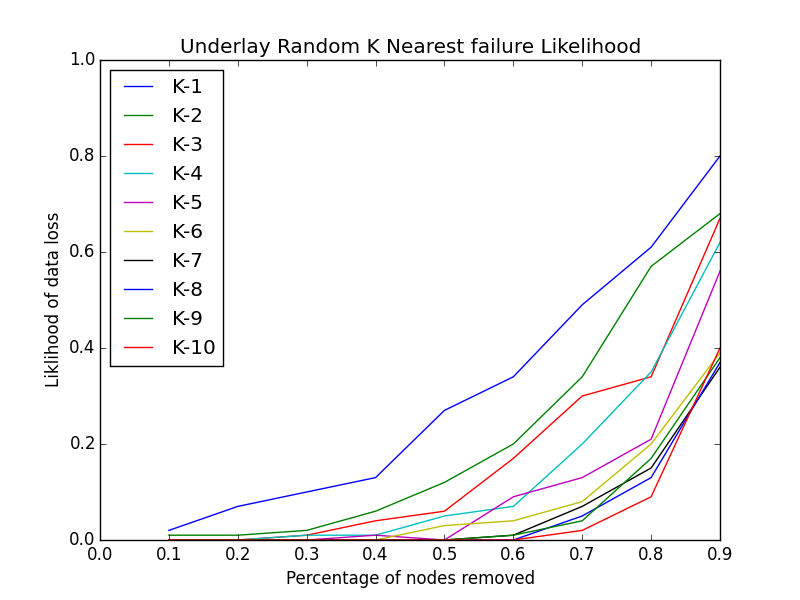
\includegraphics[width=0.5\textwidth]{figs/underlay_kad_random}
\end{figure}
\begin{figure}
	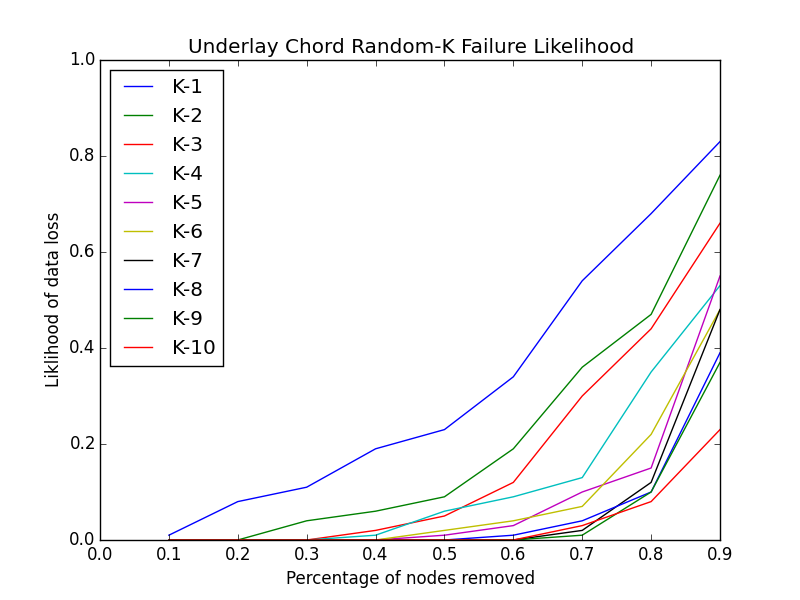
\includegraphics[width=0.5\textwidth]{figs/underlay_chord_random}
\end{figure}
\begin{figure}
	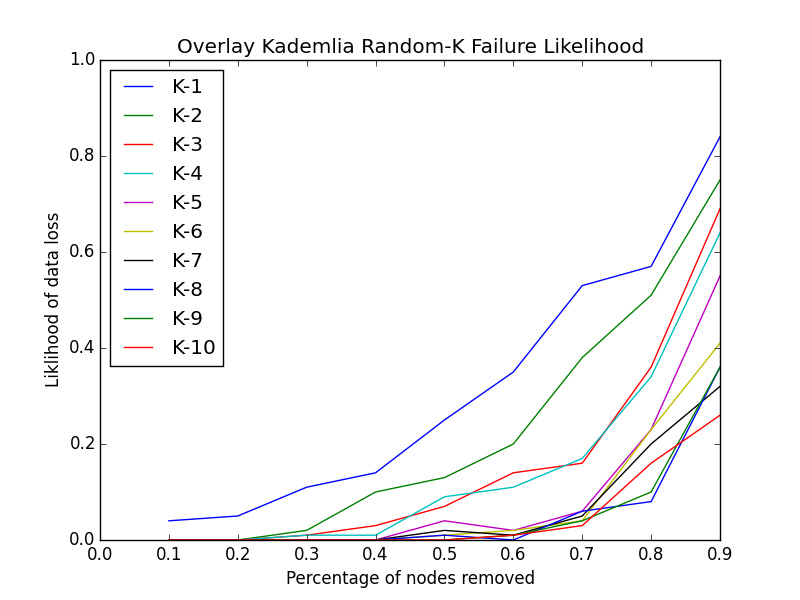
\includegraphics[width=0.5\textwidth]{figs/overlay_kad_random}
\end{figure}
\begin{figure}
	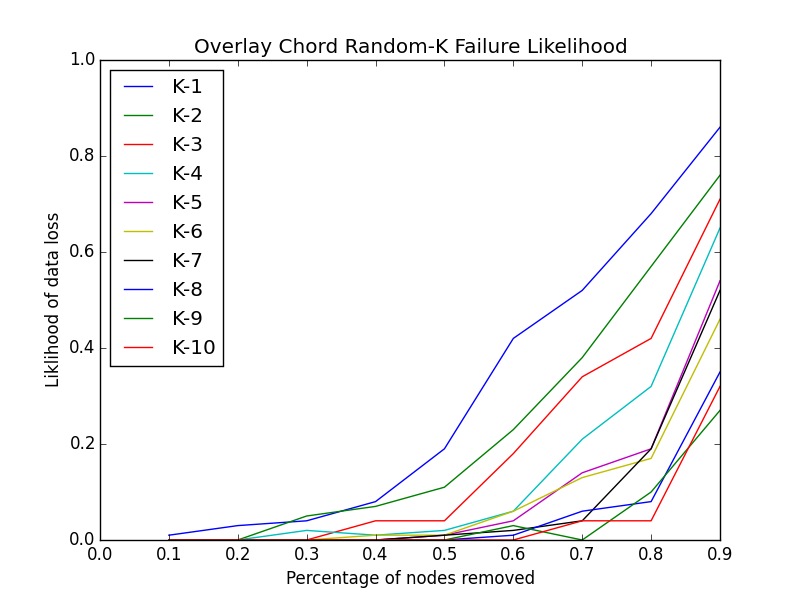
\includegraphics[width=0.5\textwidth]{figs/overlay_chord_random}
\end{figure}
\begin{figure}
	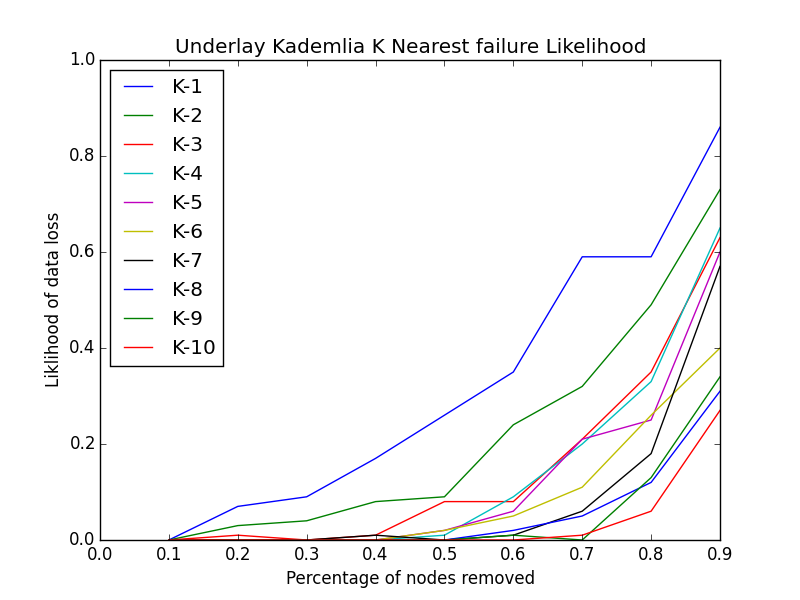
\includegraphics[width=0.5\textwidth]{figs/underlay_kad_nearest}
\end{figure}
\begin{figure}
	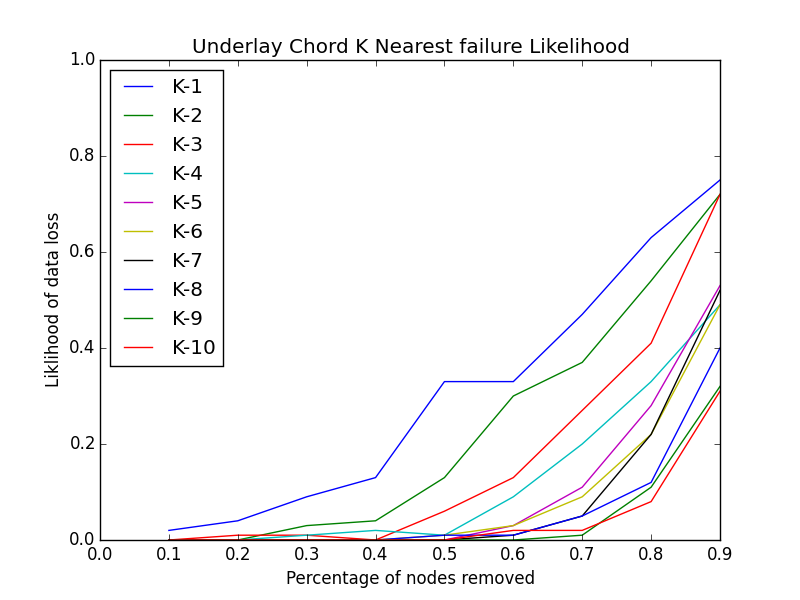
\includegraphics[width=0.5\textwidth]{figs/underlay_chord_nearest}
\end{figure}
\begin{figure}
	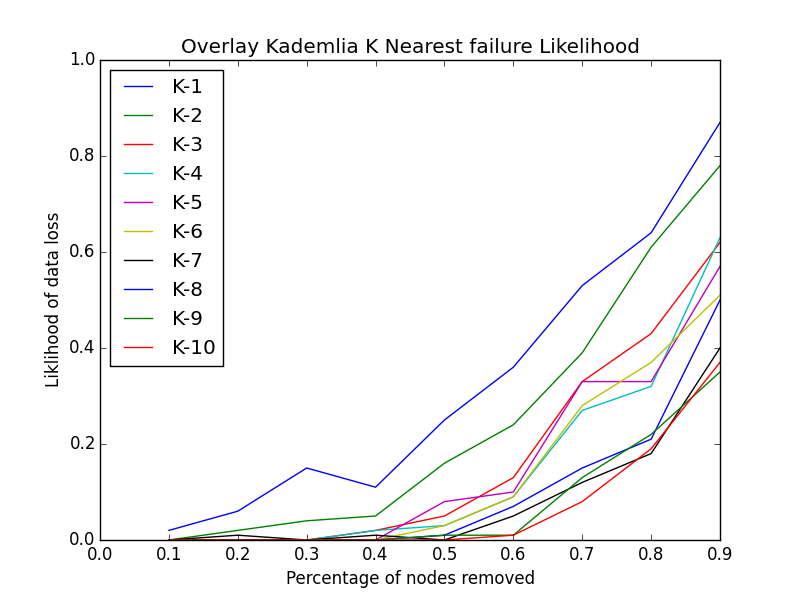
\includegraphics[width=0.5\textwidth]{figs/overlay_kad_nearest}
\end{figure}
\begin{figure}
	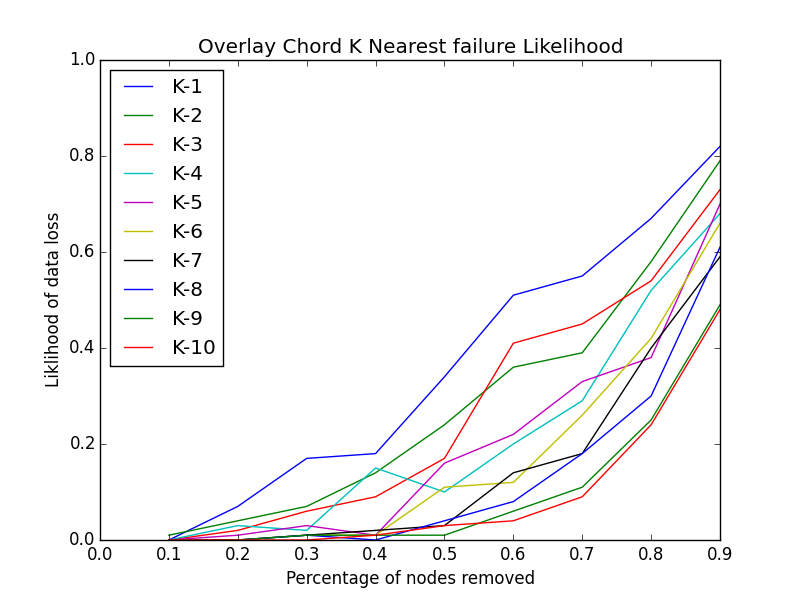
\includegraphics[width=0.5\textwidth]{figs/overlay_chord_nearest}
\end{figure}

\section{Conclusions}

Using modifications of strategies presented in 2002 by Kademlia\cite{kademlia}, which have remained largely unimplemented for the past 14 years, we can build DHT networks that can reasonably be expected to never loose records due to churn during their active use lifetime with an overhead lower than the current actively used sponsorship based strategy.

\bibliography{mine}
\bibliographystyle{IEEEtran}



\end{document}